\documentclass{article}
\usepackage{graphicx}
\usepackage{url}
\usepackage{natbib}
\usepackage{caption}
\usepackage{subcaption}
\usepackage{hyperref} % Load hyperref last
\usepackage{xcolor}
\usepackage{amsmath}
\usepackage{adjustbox}
\usepackage{makecell}
\usepackage[
    a4paper,
    total={5in, 7in}
]{geometry}

% Redefine link appearance
\hypersetup{
    colorlinks=true,
    linkcolor=black,    % Set link color to black
    filecolor=black,    % Set file color to black
    urlcolor=black,     % Set URL color to black
    citecolor=black,    % Set citation color to black
    urlbordercolor=white,  % Set URL border color to white
    citebordercolor=white, % Set citation border color to white
    linkbordercolor=white, % Set link border color to white
}

% Title
\title{Case Study 7 \bigskip \\ \textbf{Lip Products in Indonesia} \\ \large A Comprehensive Study}
\vspace{3cm} % Corrected the title spacing
\Large
\author{
    \begin{tabular}{lr}
        Arka Mukhopadhyay & B23120 \\
        Pranab Ray        & B23169 \\
        Kamal Yadav       & B23209 \\
        Arani Ghosh       & B23119 \\
        Ayuj Aryan        & B23198 \\
        Kunal Sharma      & B23079
    \end{tabular}
}
\date{\textbf{\today}}

\begin{document}
	\maketitle
	\newpage
	
	\tableofcontents
	\newpage
	
	%It is automatically generated and contains hyperlink to all the tables. See the syntax and referencing style in the text.
	\listoftables
	%\newpage
	
	%It is automatically generated and contains hyperlink to all the figures. See the syntax and referencing style in the text.
	\listoffigures
	\newpage
	
	\section{Introduction}

        \subsection{Background}
        Lips are often the unsung heroes of our skincare routine. With thinner skin, fewer oil glands, and no natural protection from the   elements, lips are prone to dryness, chapping, and cracking. To keep them looking and feeling their best, it's essential to       incorporate lip care into your daily routine. Lip products are one of the most important parts of makeup. It is even considered as  the most used beauty product in the world.
        \smallskip
        \begin{quote}
            \textit{"There are no right or wrong guidelines when it comes to lip color"}
            -- Clarissa Luna, a celebrity makeup artist in New York. 
        \end{quote}
        With a wide array of lip beauty products to choose from, finding the perfect one for you can be quite challenging. Dermatologists   advise protecting your lips from the sun with lipsticks with at least SPF 15. 
        \\ \smallskip
        
    \noindent There are a lot of Lip products and Brands available all over the world. We would like to analyze the specification of the Lip      products that are available in Indonesia's shade, brands, type and the prices that they are offering.
    
	   
	   \subsection{Objective}
    
        This research aims to determine several indicators of lip products in Indonesia based on population and sample gathered from    secondary data which are:
        \bigskip
    
        \begin{enumerate}
            \item To identify the type of data provided for lip product.
            \item To identify the average price of a popular lip product in Indonesia.
            \item To identify the famous brand of lip product in Indonesia.
            \item To identify the shades that are available for lip product in average
            \item To identify the common type of Lip Product in Indonesia.
        \end{enumerate}
    
        \subsection{Questions}
    
        \begin{enumerate}
            \item What is the type of data provided?
            \item What is the average price of a popular lip product in Indonesia?
            \item What is a famous brand for lip products?
            \item How many shades are available for some lip products on average?
            \item What is the common type of lip product in Indonesia?
        \end{enumerate}

    \section{Data and Statistics}

        \subsection{What is Data?}
        Merriam Webster describes \textbf{Data} as factual information (such as measurements or statistics) used as a basis for reasoning,  discussion, or calculation.
        \\ \\
        Before a problem is analyzed, all the information available must be converted into data. \textbf{Measurement} in the systemic process of assigning numbers to objects and their properties to facilitate the use of mathematics in studying and describing  objects and their relationships.
    
        \subsection{Types of Data}
            \subsubsection{Based on Source of Data}
            \begin{enumerate}
                \item \textbf{Primary Data}: This type of data is collected firsthand by the researcher or investigator directly from the source. It involves gathering data through methods like surveys, interviews, observations, experiments, etc. Primary data is original and specific to the research or study at hand.
        
                \item \textbf{Secondary Data}: Secondary data refers to data that has already been collected by someone else for a different purpose. This data is obtained from sources such as books, journals, government publications, websites, databases, etc. Secondary data analysis involves using existing data to derive insights or conclusions.
        
                \item \textbf{Tertiary Data}: Tertiary data is derived from primary and secondary sources. It involves the aggregation, compilation, and analysis of primary and secondary data to create new datasets or information. Tertiary data is often used for market research, trend analysis, and decision-making processes.
            \end{enumerate}
            \bigskip

            \noindent \textbf{There are several benefits of using secondary data}:
            \begin{itemize}
                \item It is cost-effective being readily available and accessible at lower costs/for free.
                \item Using existing data eliminates the need for conducting new research, allowing researchers to analyze data immediately.
                \item It contributes to a better understanding of the problem.
                \item It serves as a foundation for comparing the data gathered by the researcher across different time periods and geographies; thereby facilitating trend analysis and benchmarking.
            \end{itemize}
            
            \noindent \textbf{However, there are also disadvantages of using secondary data}:
            \begin{itemize}
                \item Secondary data rarely fits within the framework of marketing research factors since researchers have limited control over methods of collection, processing and categorization of data.
                \item The quality, precision and reliability of secondary data is unknown.
                \item Data may be out of date.
            \end{itemize}

            
            \subsubsection{Based on Levels of Measurement}

            \textbf{Quantitative data} consists of numerical or measurable values. It is typically collected through structured methods such as surveys, experiments, or measurements. Quantitative data can be analyzed statistically to identify patterns, trends, and relationships. \cite{statistics_nutshell}
            \bigskip
            
            \noindent Subcategories of Quantitative Data include:
            \begin{enumerate}
                \item \textbf{Discrete Data}: It comprises distinct, separate values that can be counted individually. Examples include the number of students in a class, the number of cars in a parking lot, etc.
        
                \item \textbf{Continuous Data}: Continuous data represents measurements that can take any value within a range. It is typically obtained through instruments like scales, thermometers, or rulers. Examples include height, weight, temperature, and time.
        
                \item \textbf{Interval Data}: Data that can be added or subtracted but not multiplied/divided. They do not have a true zero point. For example: temperature, year, etc.
                
                \item \textbf{Ratio Data}: Data that can be added, subtracted, multiplied or divided. They have a true zero point. For example: height, weight, age and so on.
            \end{enumerate}

            \noindent Data need not be inherently numeric to be useful in an analysis. For instance, male and female both are commonly used in almost any statistics report involving population but there is nothing numeric about these categories. This category of data is known as \textbf{Qualitative Data}.
            \bigskip
        
            \noindent Statisticians commonly distinguish two types of Qualitative Data:
            \begin{enumerate}
                \item \textbf{Nominal Data}: Categorical data without any inherent order or hierarchy. The categories are purely distinct labels or names. For example: types of fruits, colors, types of transportation, etc.
                
                \item \textbf{Ordinal Data}: Categorical data with a natural order or hierarchy. While the categories have a meaningful sequence, the differences between them may not be uniform. Examples include education  levels (e.g., high school, bachelor's degree, master's degree) or ratings.
                
            \end{enumerate}
            
        \subsection{What is Statistics?}

        Statistics is the science of data. This involves collecting, classifying, summarizing, organizing, analyzing, and interpreting data. It involves methods for designing experiments and surveys, gathering data, and drawing conclusions from that data.  

        \noindent Statistics is widely used in various fields such as science, business, economics, engineering, social sciences, and many others. It helps in making informed decisions, predicting outcomes, testing hypotheses, and understanding patterns and trends in data.

        \noindent There are two kinds of Statistics:

        \begin{enumerate}
            \item \textbf{Inferential Statistics}: Statistical inference is the science of characterizing or making decisions about a population by using information from a sample drawn from that population. This includes hypothesis testing, confidence intervals, and regression analysis.

            \item \textbf{Descriptive Statistics}: Descriptive statistics uses data that provides a description of the population either through numerical calculated graphs or tables. It provides a graphical summary of data. It includes:
            \begin{itemize}
                \item Measures of Central Tendency (Mean, Median and Mode)
                \item Measures of Variability (Range, Variance, Dispersion, and so on)
            \end{itemize}
        \end{enumerate}

    \section{Sampling}
        \subsection{Key Terminologies}
        \begin{enumerate}
            \item \textbf{Population}: The population refers to the entire group of individuals, objects, or events who represent a characteristic. A \textit{census} study involves the entire population.

            \item \textbf{Sample}: A sample is a subset of the population selected for observation or measurement.

            \item \textbf{Sampling}: Sampling is the process of selecting a \textit{sample} from the \textit{population} to make statistical inferences and estimate population characteristics.

            \item \textbf{Sampling Frame}: A sampling frame is a list of all the individuals, objects, or events in the population from which the sample will be selected.
        \end{enumerate}

        \subsection{Sampling Schemes}

        A good sample must reflect all the characteristics (of importance) of the population. A sample that accurately reflects its population characteristics is called a \textit{representative sample}. A sample that is not representative of the population characteristics is called a \textit{biased sample}. The reliability or accuracy of conclusions drawn concerning a population depends on whether or not the sample is properly chosen so as to represent the population sufficiently well. \cite{stats_applications}

        \noindent The selection of a sampling method depends on factors such as the nature of the investigation, the availability of sampling frames (lists of population members), financial resources, desired accuracy level, and data collection method (e.g., questionnaires or interviews). 

        \noindent Common sampling techniques include:

        \begin{enumerate}
            \item \textbf{Simple Random Sample}: A sample selected in such a way that every element of the population has an equal chance of being chosen is called a simple random sample.
            
            \item \textbf{Systematic Sampling}: A systematic sample is a sample in which every $k^{th}$ element in the sampling frame is selected after a suitable random start for the first element with the population listed in some defined order.
            
            \item \textbf{Stratified Sample}: Here, a sample obtained by stratifying (dividing into non-overlapping groups) the sampling frame based on some factor(s) and then selecting some elements from each of the strata. A population with N elements is first divided into 's' sub-populations, then a sample is drawn from each sub-population independently. 

            \item \textbf{Cluster or Area Sampling}: In cluster sampling, the sampling unit contains naturally existing groups of elements called clusters instead of individual elements of the population. A cluster is an intact group naturally available in the field.
            
        \end{enumerate}
        \subsection{Bias in Sampling}

        Sampling bias refers to the systematic error introduced into a sample as a result of the sampling method. It occurs when some members of a population are systematically more likely to be selected in a sample than others, leading to inaccurate or misleading conclusions and limits the generalizability of the findings. \cite{statistics_nutshell} \cite{scribbr_bias}

        \noindent The following are some common types of sampling biases:

        \begin{enumerate}
            \item \textbf{Selection Bias}: Selection bias exists if some potential subjects are more likely than others to be selected for the study sample; usually due to the sampling process.

            \item \textbf{Volunteer Bias}: Volunteer bias refers to the fact that people who volunteer to be in studies are usually not representative of the population as a whole. For this reason, results from entirely volunteer samples might be considerably different from those who do not volunteer.

            \item \textbf{Non-Response Bias}: Non-response bias occurs when individuals selected for the sample do not respond to the survey or study. This can lead to under-representation of certain groups in the sample, skewing the results.
        \end{enumerate}
        \begin{figure}[htbp]
		      \centering
		      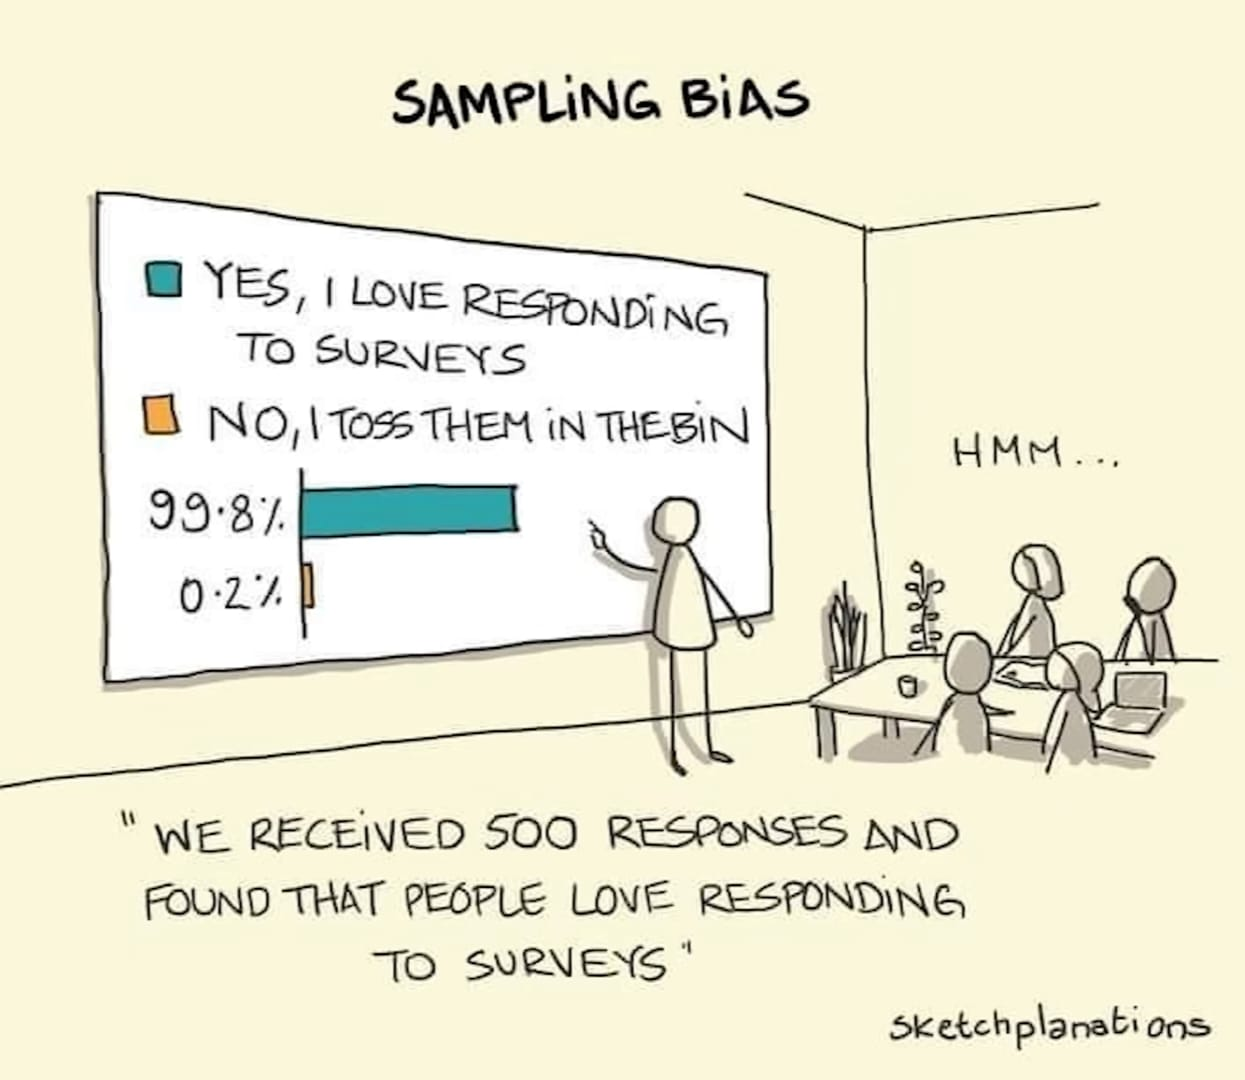
\includegraphics[scale = 0.25]{../images/sampling_bias_meme.jpeg}
		      \caption{Example of Sampling Bias}
		      \label{Sampling_Bias}
	    \end{figure}
          \section{Methodology}
        \subsection{Data Collection}
            In our study, to minimize time spending, secondary data is used as the resources since there are millions of lip products in Indonesia.

            \noindent Stratified sampling method is used to determine the sample in this research by dividing the population into subgroups based on the factors like brands, type, products, etc. 

        \subsection{Data Analysis}
    
    \section{Raw Data}
    Here's the table that would be used for this study:
    \newgeometry{left=1cm,right=1cm}
\begin{table}[htbp]
    \centering
    \caption{Raw Data for Study}
    \label{tab:Table_Raw}
    \begin{tabular}{ccccc}        \hline
        \textbf{Lip Product}                    & \textbf{Brand}    & \textbf{Type of Lip Product} & \textbf{Shades} & \textbf{Price} \\ \hline
        NIVEA LIP BALM SOOTHE \& PRTECT         & Beiersdorf        & Stick                        & 2               & 50000          \\
        Extra lip tint                          & Bobbi Brown       & Stick                        & 10              & 711636         \\
        Perfect Matte Lip Coat                  & Dear Me Beauty    & Liquid                       & 6               & 129000         \\
        Creamytint                              & Emina             & Liquid                       & 5               & 46000          \\
        magic potion lip tint                   & Emina             & Liquid                       & 5               & 50000          \\
        Squeeze me up Lip Matte                 & Emina             & Liquid                       & 4               & 58000          \\
        Smoochies Lip balm                      & Emina             & Solid                        & 1               & 32000          \\
        Matte Lip Liquid                        & ESQA              & Liquid                       & 7               & 165000         \\
        Dear Darling Water gel tint             & Etude House       & Liquid                       & 3               & 55000          \\
        Organic lip balm                        & Eucalie           & Stick                        & 1               & 79000          \\
        lip and cheek dual use liquid           & Focallure         & Liquid                       & 10              & 38000          \\
        Melted Matte Lip                        & Goban Cosmetics   & Liquid                       & 6               & 130000         \\
        Sheen. Tinted lip balm + UV filter      & HALE.             & Stick                        & 4               & 98000          \\
        Urban Lip Cream Matte                   & Implora           & Liquid                       & 20              & 25000          \\
        Beauty Lip \& Cheeck Crayon             & Indoganic         & Crayon                       & 2               & 129000         \\
        Vivid oil tint                          & Innisfree         & Liquid                       & 4               & 104000         \\
        Metallic Lip Cream                      & Inul Beauty       & Liquid                       & 5               & 89000          \\
        Infalible Pro Matte Lip Liquid          & L'oreal           & Liquid                       & 9               & 150000         \\
        Rouge Signature Liquid Matte Lipstick   & L'oreal           & Liquid                       & 14              & 151376         \\
        Color Riche Matte                       & L'oreal           & Stick                        & 8               & 354267         \\
        Intense Matte Lip Cream                 & Liquid            & Liquid                       & 12              & 119000         \\
        Longlasting Matte Lip Cream Metalic     & LT Pro            & Liquid                       & 3               & 109900         \\
        Ultra Light Lip Stain                   & Luxcrime          & Liquid                       & 8               & 79000          \\
        Airy lip mousse                         & Luxcrime          & Liquid                       & 8               & 109000         \\
        Dew tinted 6hr lip moisturizer          & Mad for Makeup    & Stick                        & 6               & 109000         \\
        magnifique lip tint                     & Madame Gie        & Liquid                       & 6               & 33000          \\
        Brilliant Glaze Lip Liquide             & Madame Gie        & Liquid                       & 6               & 35000          \\
        Moist Velvet \& Smooth Lip Liquide      & Madame Gie        & Liquid                       & 6               & 15765          \\
        Hydrastay lip whip                      & Makeover          & Liquid                       & 12              & 119000         \\
        Powestay Transfer Proof Matte Lip Cream & Makeover          & Liquid                       & 12              & 135000         \\
        Sensational Liquid Matte                & Maybelline        & Liquid                       & 19              & 66,023         \\
        color sensational lip tint              & Maybelline        & Liquid                       & 19              & 45000          \\
        Super Stay Matte Ink                    & Maybelline        & Liquid                       & 19              & 239571         \\
        Color sensational the powder mattes     & Maybelline        & Stick                        & 24              & 88900          \\
        Hydra Lip Cheek Tint                    & Mineral Botanica  & Liquid                       & 4               & 51900          \\
        the one A-Z lip balm SPF 25             & Oriflame          & Stick                        & 2               & 149000         \\
        Lip Cream                               & PIXY              & Liquid                       & 16              & 55000          \\
        2 in 1 color tint                       & Purbasari         & Liquid                       & 3               & 51900          \\
        Lip Cream Series                        & Raiku             & Liquid                       & 13              & 118000         \\
        SUEDED! Lip \& Cheek Cream              & Rollover Reaction & Liquid                       & 12              & 109000         \\
        Juicy Lip Balm                          & Rose All day      & Stick                        & 3               & 119000         \\
        Lip Color                               & Runa Beauty       & Stick                        & 5               & 138000         \\
        Lip Care                                & Sensatia Botanica & Liquid                       & 5               & 80000          \\
        Coconut lip sleeping balm               & Tiff Body         & Liquid                       & 1               & 88000          \\
        delight tony tint                       & Tony Moly         & Liquid                       & 3               & 49000          \\
        Exclusive Matte Lip Cream               & Wardah            & Liquid                       & 24              & 66500          \\
        Colorfit Velvet Matte Lip Mousse        & Wardah            & Liquid                       & 14              & 79000          \\
        Everyday Moisture Lip nutrition         & Wardah            & Stick                        & 2               & 28500          \\
        Color Fit Ultralight Matte              & Wardah            & Stick                        & 5               & 47500          \\
        The Simplicity Love You tint            & Y.O.U             & Liquid                       & 4               & 45100          \\
    \end{tabular}
\end{table}
\restoregeometry
    
    \section{Sampled Data}  
        \subsection{On Basis of Brands}
        Table with the sampled data on the basis of brands:  
    \section{Scripts}
    \section{Inference}

    % Bibliography
	\newpage
	\bibliographystyle{unsrt}
	\bibliography{references}
    \addcontentsline{toc}{section}{\refname}

    \newpage
    \newgeometry{left=1cm,right=1cm}
\begin{center}
    \section*{Contributions}
\end{center}
\begin{table}[htbp]
    \centering
    \caption{Contributions of the authors}
    \label{tab:Table_Contri}
    \begin{tabular}{|c|c|c|c|c|c|}
        \hline
        \textbf{\thead{Name}} & \textbf{\thead{Roll No.}} & \textbf{\thead{Contribution \\ in Report Writing}} & \textbf{\thead{Contribution \\ in Analysis}} & \textbf{\thead{Details of use \\ of web resources/\\Codes/AI tools, etc.}} & \textbf{\thead{Overall \\ Contribution \\ to work done}} \\ \hline
        Arka Mukhopadhyay & B23120 & Remaining & \begin{tabular}{@{}c@{}}Grouping products \\ by brands and type \end{tabular} & \begin{tabular}{@{}c@{}} CSV to LaTeX \\ table converters \end{tabular} & 16.8 \\ \hline
        Pranab Ray & B23169 & \begin{tabular}{@{}c@{}}Data Analysis \\ Inference\end{tabular}& \begin{tabular}{@{}c@{}} Remaining \end{tabular} & \begin{tabular}{@{}c@{}}ChatGPT and Gemini \\ to refine writeups \end{tabular} & 16.8 \\ \hline
        Kamal Yadav & B23209 & Data Collection & \begin{tabular}{@{}c@{}}Collecting \\ Indian Data \end{tabular} & - & 16.6 \\ \hline
        Arani Ghosh & B23119 & - & \begin{tabular}{@{}c@{}}KDE and \\ Descriptive Statistics \end{tabular} & \begin{tabular}{@{}c@{}}GitHub Copilot \\ to beautify graphs \end{tabular} & 16.6 \\ \hline
        Ayuj Aryan & B23198 & Data Collection & \begin{tabular}{@{}c@{}}Collecting \\ Indonesian Data \end{tabular} & - & 16.6 \\ \hline
        Kunal Sharma & B23079 & Data Collection & \begin{tabular}{@{}c@{}}Collecting \\ Indian Data \end{tabular} & - & 16.6 \\ \hline
    \end{tabular}
\end{table}
\restoregeometry
	
\end{document}